\documentclass[conference]{IEEEtran}
\IEEEoverridecommandlockouts
% The preceding line is only needed to identify funding in the first footnote. If that is unneeded, please comment it out.
\usepackage{cite}
\usepackage{amsmath,amssymb,amsfonts}
\usepackage{algorithmic}
\usepackage{graphicx}
\usepackage{textcomp}
\def\BibTeX{{\rm B\kern-.05em{\sc i\kern-.025em b}\kern-.08em
    T\kern-.1667em\lower.7ex\hbox{E}\kern-.125emX}}
\begin{document}

\title{CENG435 Group 60 TP Part-2 Report\\
%{\footnotesize \textsuperscript{*}Note: Sub-titles are not captured in Xplore and
%should not be used}
\thanks{}
}

\author{\IEEEauthorblockN{\textsuperscript{} Kadir Burak Tokmak}
\IEEEauthorblockA{\textit{} 
\textit{ID :2036200} \\
}
\and
\IEEEauthorblockN{\textsuperscript{} Emrah Kosen}
\IEEEauthorblockA{\textit{}
\textit{ID:1942317}\\
}

}

\maketitle





\section{Introduction}
\large

For second part of our project we are working with the same topology consisting of 5 nodes with total of 8 links. Each link has its own interface on the nodes and their subnet contains 2 hosts each. \\
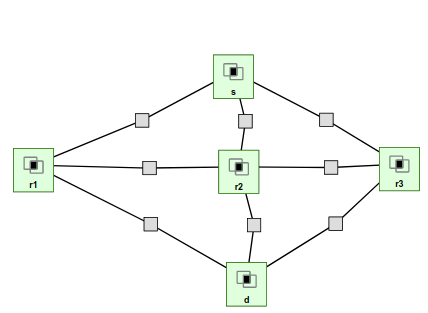
\includegraphics[width = 90mm, height = 80mm]{topologyp2.png}\\ \qquad \\


Topology links contents can be shown as:\\

$\bullet$R1-R2 link: 10.10.8.0/24 Subnet with 100kbs bandwidth\\

$\bullet$R2-R3 link 10.10.6.0/24 Subnet with 100kbs bandwidth\\

$\bullet$R1-D link 10.10.4.0/24 Subnet with 1000kbs bandwidth\\

$\bullet$R2-D link 10.10.5.0/24 Subnet with 1000kbs bandwidth\\

$\bullet$R3-D link 10.10.7.0/24 Subnet with 2000kbs bandwidth\\

$\bullet$R1-S link 10.10.1.0/24 Subnet with 1000kbs bandwidth\\

$\bullet$R2-S link 10.10.2.0/24 Subnet with 1000kbs bandwidth\\

$\bullet$R3-S link 10.10.3.0/24 Subnet with 2000kbs bandwidth\\

Connections to this topology is made via ssh connections and this topology is working on virtual machines to operate.\\


For the second part of the project reliable data transfer between S and D nodes needs to be implemented. For this data transfer UDP protocols and sockets are going to be used. For reliable data transfer checksum for the packets and file as a whole needs to made so that file is transferred without corruptions or loss. For data transfer between S-D S-R1-D, S-R2-D, S-R3-D routes are going to be used. Project consists of two experiments for experiment 1 S-R3-D path will be used for data transfer. For experiment 2 S-R2-D and S-R1-D routes are going to be used with multihoming. Any of these 2 links can be downed while transferring data and scripts should cover for that. Pipelining is also implemented for scripts and used in both experiments.\\

A file will be send for each experiment. Experiments will be performed with different network configurations. \%5, \%15,\%38 loss rates are going to be implemented in all links of the data transfer topology and experiments 1,2 will be done for each loss emulation. Packet size sent by UDP sockets must be smaller than 1000bytes\\ 

Design of the custom rdt protocol and implementation of it will be discussed also results times are going to be analyzed and discussed after the experiments.    \\ \quad \\

\section{Design}

Implementing reliable data transfer requires a checksum and acknowledgment based communication needs to be implemented. For transferring data packet window is going to be use with a similar approach to selective-repeat method. A window needs to be completed before moving into another window of packets. In the window received packets are going to be flagged and only other packets will be sent. \\

Packets received will be controlled for checksum before updating that packet received status. After cheksum is confirmed and packet is not corrupted it is saved in window and will wait for all window to finish.\\
 
Write to file happens after a window is finished all data in the window will be written to file. If last received window is not a full window, after not getting any package it will timeout and write the last part of the data to file. \\

Acknowledgment of the sequence is important for script to continue working and send new windows even though data is received  by the client side , ack message is required for server to know that how much of the window did client received without problem. In a data sent and acknowledgment received situation a packet needs to go through links 4 times since there are R1-R2-R3 nodes in the routes. So with a \%5 loss at every link project will have ~\%19 chance of losing the packet in the transfer whether its the data that is being sent or the acknowledgment. At \%15 loss at every link this chance will be  ~\%48. Chance to lose a packet will be ~\%85 for \%38 loss  at every link. For compensate the loss of \%85 of our packets high timeout will be implemented to make sure that file transfer is not over because of packet losses. Timeout will still work for if a connection of a link is down or if file transfer end abruptly for any reason. \\

Messages are send in packets with the sequence number, cheksum and data. Big parts of the packets will be data but checksum and sequence number will be used in the start of messages as rdt measures. Implementation of these will be detailed later.\\

For R1-R2-R3 simple redirector scripts will be used. These node will re-direct messages between S-D and will timeout if they are not used.\\ \qquad \\

 

\section{Implementation}

For implementations of the scripts python language is used. Scripts are executed with python and socket,time libraries are used for the scripts.\\

In the socket library UDP sockets are defined and bind to corresponding IP Address and port from IP table. IP tablse used in the scripts:\\

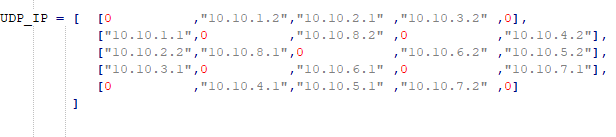
\includegraphics[width = 90mm, height = 30mm]{iptable.png}\\ \qquad \\

Nodes S-D-R1-R2-R3 have their index numbers as 0-1-2-3-4\\

To reach destination IP address for sending packet from S to R1  Matrix [0][1] is used and for listening to R1 at S Matrix [1][0] is used.\\

Ports for sending receiving defined same for R1-R2-R3 for both S-D nodes.\\

Ports 10001 used for R1, ports 10002 used for R2, ports 10003 used for R3\\

First a window is implemented with an array. Our window size is 10 and our segment size chosen to be 980 since packet size cant be bigger than 1000. Our actual packets will be bigger than 980 with the header, checksum and sequence number information. Window size is filled with data from the "input.txt" file. 980x10=9800bytes maximum data for our window. window is initialized to hold -1 in all members showing that it has no data inside.\\

Window condition array is also implemented to keep track of the segments in windows. Initial values of these array members also -1. -1, 0 ,1 flags are used in node S(server). 
 -1 means it is sent,
 0 means it is sending but not acknowledged yet,
 1 means ready to send.\\
 
 For S node two functions are defined one as packet sender other as window updater. Window updater checks the global variables and if a window is completely sent it fills window with the correct offset of the file. Offset incremented by segment size every time segment is given to window. Window updater makes the correct initialization and fillings for both array script is using.\\
 
Pipelining and multihoming for the project done with threading and with the help of the window arrays at packet sender function. \\

Scripts at both S-D will work according to argument they receive at terminal. If argument "1" for experiment 1 is given only one thread for R3 will be opened for sending and receiving. For  experiment 1 there is no multihoming. If argument "2" is received for the scripts threads for both R1-R2 will be opened and will work with window updater thread to implement multihoming functionality to the project. Packet sender function engages with window condition array and looks for value 1 to pick a segment and send. Until an acknowledgment is received or packet timed out condition will be 0. If sender function receives acknowledgment for the packet it sent then it will update the window condition as -1. If a timeout happens corresponding sequence will be updated back to 1 and will be available to pickup for other threads. \\

Before sending data its packed into three objects which will be used in receiving end "D". First 2 bytes (16bits) will be the chekcsum information of the data. Third byte will be the sequence number and rest of the packet will be the file data. \\

To calculate checksum add every 16bit algorithm is used. After 16bit result cheksum is obtained function returns it for our usage in both client and server nodes. Same function is used for both nodes to achieve correct result. Function is defined in a different python file which is imported as library in our node S-D that will use the checksum function with the data.\\

Pipelining also implemented by sending more than one segment without receiving acknowledgment and after receiving acknowledgment sequence packet sender function only sends back packets with flags 1 which means their acknowledgment is not received and needs to be sent again. \\

Threadding for send packet also allows the project for script to work on more than two transferring nodes for multihoming. Just adding another thread with the addresses from the topology will allow the script to run with more nodes with  multihoming.\\

For D node two main functions are implemented which will work in threads to fulfill the needs of the project. One the function is window updater and file writer. This function will work with two arrays for window implementation. One of the array will hold the data received and other array will hold the window condition. Flag "-1" will mean that that packet of the window is not received yet and flag "1" will mean packet is received for corresponding segment in window. When a window is fully received and flag is set this function will write its contents to output.txt or output2.txt depending on the argument its called with. After a window is written to file new window is opened up for new segments to be received.  \\

Second function for the D node is get packet function. This function will get packets from R1-R2-R3 nodes with the threading implementation. If argument 1 is used this function is threaded by only R3 destination on the other hand if an argument 2 is given to script it will use R2 and R1 destinations in two threads. This function will look for a packet to receive before timing out. After a packet is received first 2 bytes of the packet will be compared to checksum of the data part of the packet. After calculating the checksum of data and looking at first 2 bytes if they are a match function sets the flag for that packet to be taken and starts sending packets with the acknowledged sequence numbers. These acknowledgments sent until timeout. With the correct timeout implementation for our \%38 loss at every link as worst case scenario our acknowledgments are sure to be sent to S node which will terminate before D node. After updating the flags and sequences its corresponding segment window will be finished and window updater is awaited for new window.\\

Scripts in transfer nodes will be simple as their only duty to send the packet received to other end of their connection. Checksum here would be useless since packet can get lost or corrupted while re-directing. All re-direct packet scripts works with two threads. One of them re-directing packets from S to D other re-directing packets from D to S.\\

Nodes D-R1-R2-R3 are working under a timeout rule which determines their if their work is finished or not. For the worst case scenario 20 seconds timeout implemented to be safe since a packet may not reach its destination after repeats of 10-15 seconds with a \%38 loss at every link which means we can not see the response of \%85 of our sent packets. After timeouts re-directs at R1-R2-R3 are finished. Also write to file of last segments are done with the timeout at the D.\\

Multihoming allows us to transfer packets from both R1-R2 at the same time and can be seen in action in the screenshot at Appendix 1. While S-D nodes are printing for window and sequence information R1-R2 nodes are printing which destination they sent a data towards. Destinations are in the form of IP Addresses.\\

As discussed in introduction links can be downed during multihoming and file transfer should happen without loss after such a situation. Implementation of pick available packet and set to available if timeout happens in our sendpacket function at node S overcomes the situation of this link down. Even a link is down thread corresponding to that link will recieve timeout and give up the segment in window to be transmitted but other threads. With \%38 loss at all links we cut the re-direction script of R2 after 2 seconds to test if our link down protocols worked. Rest of the file is sent by only R1 and total time for the operation is increased as a result. Screenshot of this event can be seen in Appendix 2.\\

Since implementation of the scripts seemed to work fine with our small tests we moved on to making experiments with \%5 loss \%15 loss and \%38 loss. To appply these loss rate on each nodes "tc qdisc" network emulation commands are used at every for corresponding ethernet interfaces. Two interfaces need to be edited on R1-R2-R3 nodes which are corresponding to S and D nodes. Three interfaces are to be edited in S-D nodes corresponding to R1,R2 and R3 node links. With the help of ifconfig command ethernet interface names are identified to be edited. For R1 eth1 and eth2, for R2 eth2 and eth4 for R3 eth1 and eth2 for S eth1,eth2 and eth3 for D eth1,eth2,eth3 needs to be edited. \\

Used command to edit interfaces at start in R1 :\\ 

sudo tc qdisc add dev eth1 root netem loss 5\% delay 3ms \\
sudo tc qdisc add dev eth2 root netem loss 5\% delay 3ms \\

For other values of loss values same code is used with "change" instead of "add" and interfaces are manipulated to have \%15 and \%38 losses.\\

Experiments done first at \%5 loss then all interfaces are added \%15 loss and lastly experiments are done at \%38 loss at all links. Every experiment repeated 5 times for the production of result graph of loss versus time for both experiments.\\

Experiment 1 with \%5 loss of sending 5000000 bytes file took 250~ seconds since the results can be scaled with the size of the file in our scripts we decided to use Term Project description as input.txt . File is 25564 bytes results can be scaled with result*195.6~ to reach expected results. Following graphs will show the time for spent for file with 25564 bytes content. ( Multiple experiments with original file would have taken hours to perform). \\

After 5 repeats of these experiments with file of 25564 bytes file received at the D node is checked and file was complete without corruption and same file size. For experiment 1 and experiment 2 results of the tests are made into  graphs with \%95 confidence intervals which can be seen below:\\

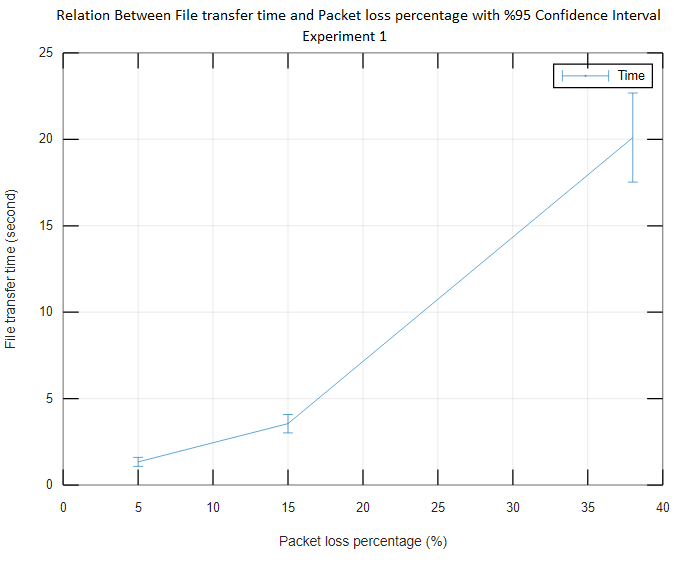
\includegraphics[width = 90mm, height = 80mm]{exp1_confidence.png}\\ \qquad \\
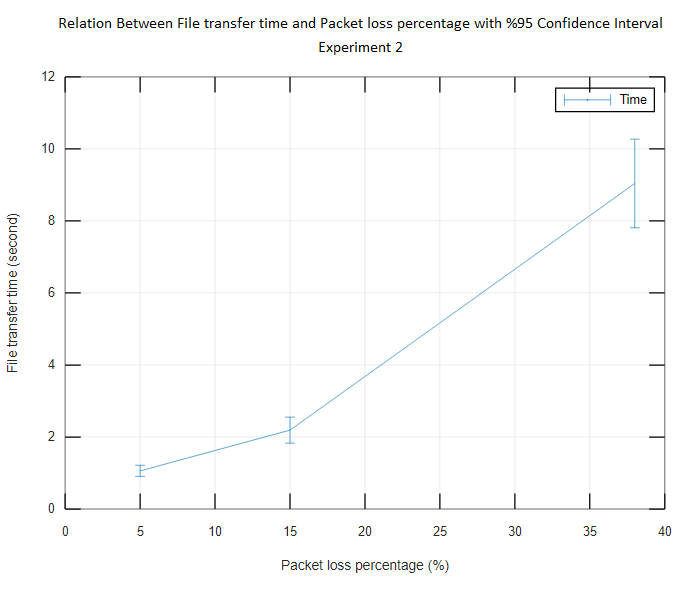
\includegraphics[width = 90mm, height = 80mm]{exp2_confidence.png}\\ \qquad \\

Experiment results can also be found in results.txt. From the results we can identify that for both of the experiment types file transfer time increases with the packet loss increase. As the packet loss increase we can see an increase of differentiation in our results. Multihoming protocol performs better compared to single node transfer as the packet loss increases. This effect can be explained by our multihoming with two nodes we double the chances of our packets reaching destination by sending and receiving more packets. We can see that with the flexibility of our code if we include R3 into multihoming file transfer times will be faster than experiment 2. \\ \qquad \\



\section{Conclusion}

Part 2 of the project ended with the analysis of the results we got from both experiments at different loss states of the packets. Implementation of the multihoming and pipelining allowed file transfer to be more efficent. RDT is implemented with these methods and with the help of checksum controls, window and segment management with acknowledgment messages. Impacts of multihoming and packet loss emulations seen with hands on experiments. Please take a look at the attached files and ReadMe.txt for more information about project part 2 and script implementation. \\ \qquad \\

\vspace{\baselineskip}
\vspace{\baselineskip}
\vspace{\baselineskip}
\vspace{\baselineskip}
\vspace{\baselineskip}
\vspace{\baselineskip}
\vspace{\baselineskip}
\vspace{\baselineskip}
\vspace{\baselineskip}
\vspace{\baselineskip}
\vspace{\baselineskip}
\vspace{\baselineskip}
\vspace{\baselineskip}
\vspace{\baselineskip}
\vspace{\baselineskip}
\vspace{\baselineskip}
\vspace{\baselineskip}
\vspace{\baselineskip}

\section{Appendix}

Appendix 1:\\

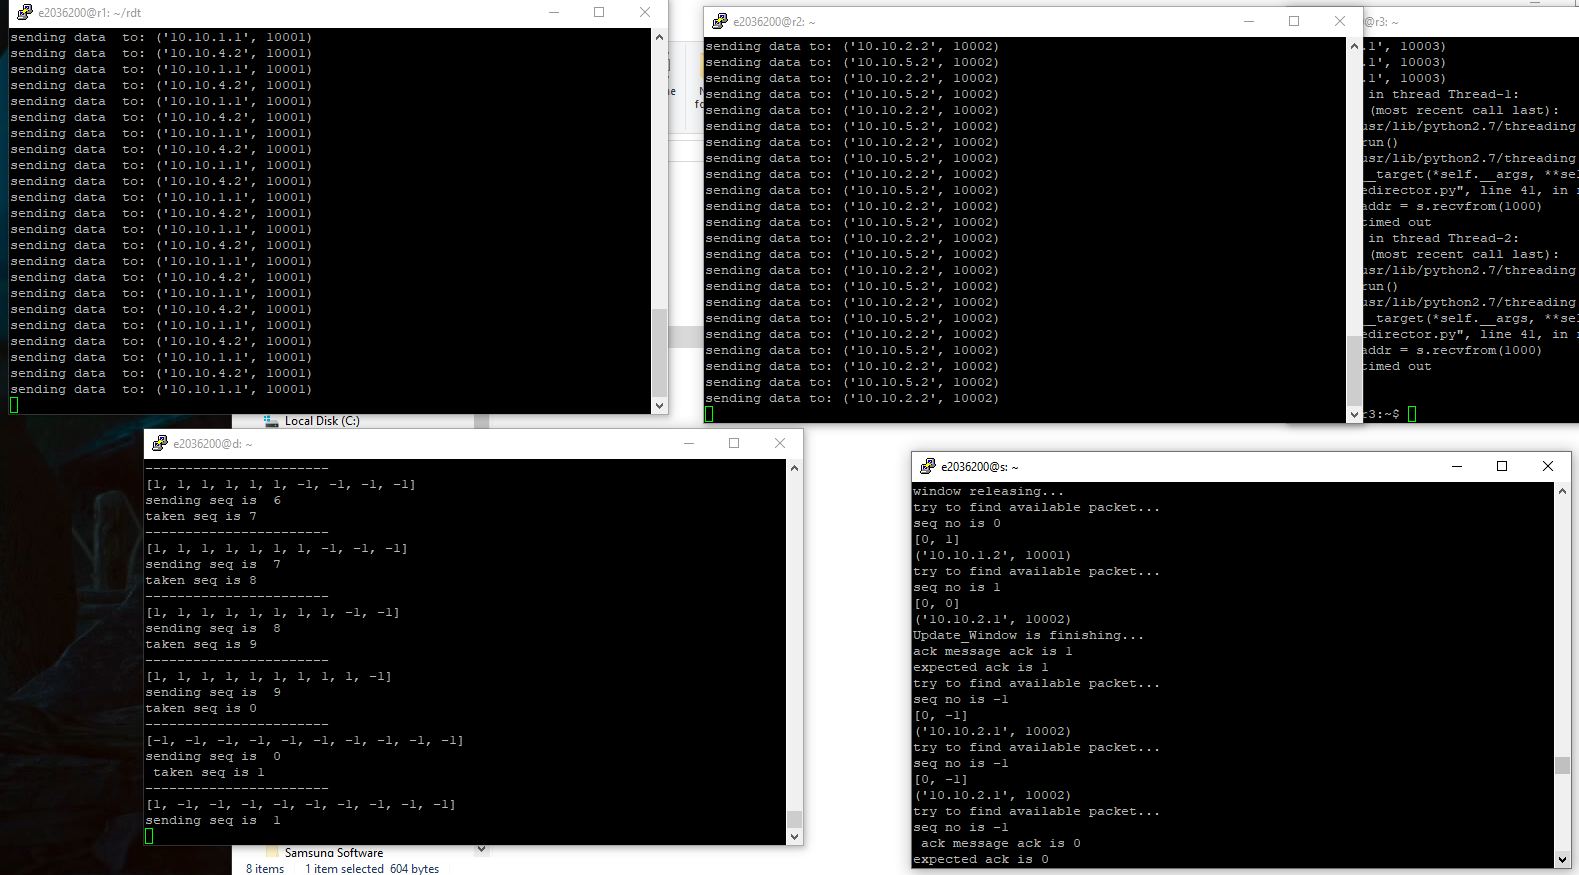
\includegraphics[width = 145mm, height = 90mm]{multihoming2.png} \\ \qquad \\



Appendix 2:\\

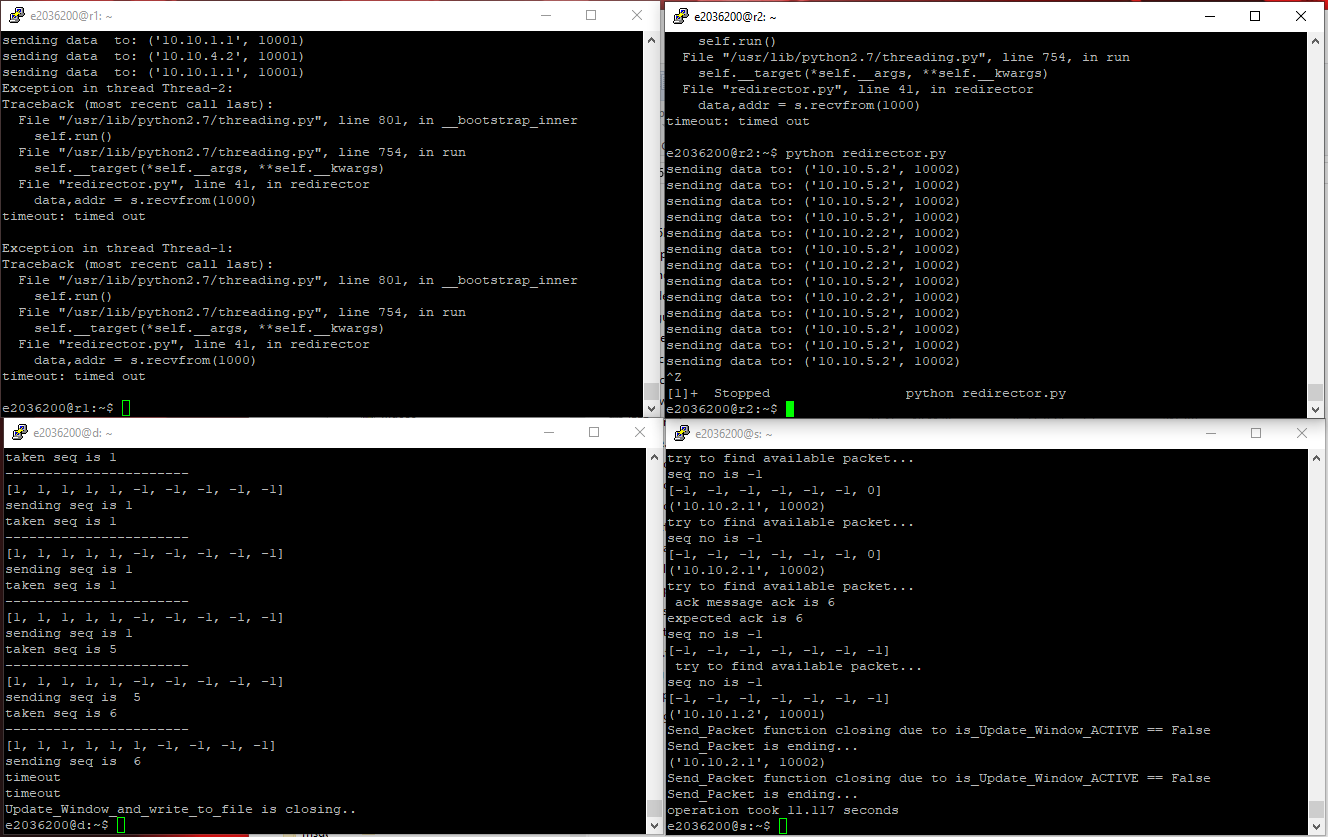
\includegraphics[width = 145mm, height = 90mm]{multihoming_linkdown.png} \\ \qquad \\

\end{document}
